\part{Types and Subtyping}

\section{Types}

\subsection{Type Systems}
\begin{definition}[Type System]
 A type system is a tractable syntactic method for
proving absence of certain program behaviors by
classifying phrases according to the kinds of values
they compute.
\end{definition}
\begin{description}
 \item[Syntactic] Rules are based on form, not behavior
 \item[Phrases] Expressions, methods, etc... of a program. 
 \item[Kinds of values] Types
\end{description}

\subsection{Weak and Strong Type Systems}
\begin{description}
 \item[Untyped Languages] Do not classify values into types.\\
  Example: Assembler
 \item[Weakly-typed Languages] Classify values into types, but do not srictly enforce additional restrictions.\\
  Examples: C, C++
 \item[Strongly-typed Languages] Enforce that all operations are applied to arguments of the appropriate types.\\
  Examples: C\#, Eiffel, Java, Python, Scala, Smalltalk
\end{description}

Strongly-typed languages prevent certain
erroneous or undesirable program behavior
Comparison between strong and weak typing:
\lstset{language=C}
\begin{lstlisting}[caption=C Example]
int main( int argc, char** argv ) { 
  int i = ( int ) argv[ 0 ]; 
  printf( "%d", i ); 
} 
\end{lstlisting}
\lstset{language=Java}
\begin{lstlisting}[caption=Java Example]
int main( String[ ] argv ) {
  int i = ( int ) argv[ 0 ];
  System.out.println( i );
}
\end{lstlisting}
The Java example results in a Compile-time error.

\subsection{Types}
\begin{definition}[Types]
A type is a set of values sharing some properties. A value v has type T if v is an element of type. 
\end{definition}
\begin{description}
 \item[Nominal Types] are based on \emph{type names}\\
  Examples: C++, Eiffel, Java, Scala
 \item[Structural Types] are based on \emph{availability of methods and fields}\\
 Examples: Python, Ruby, Smalltalk
\end{description}

\begin{figure}[H]
  \centering
    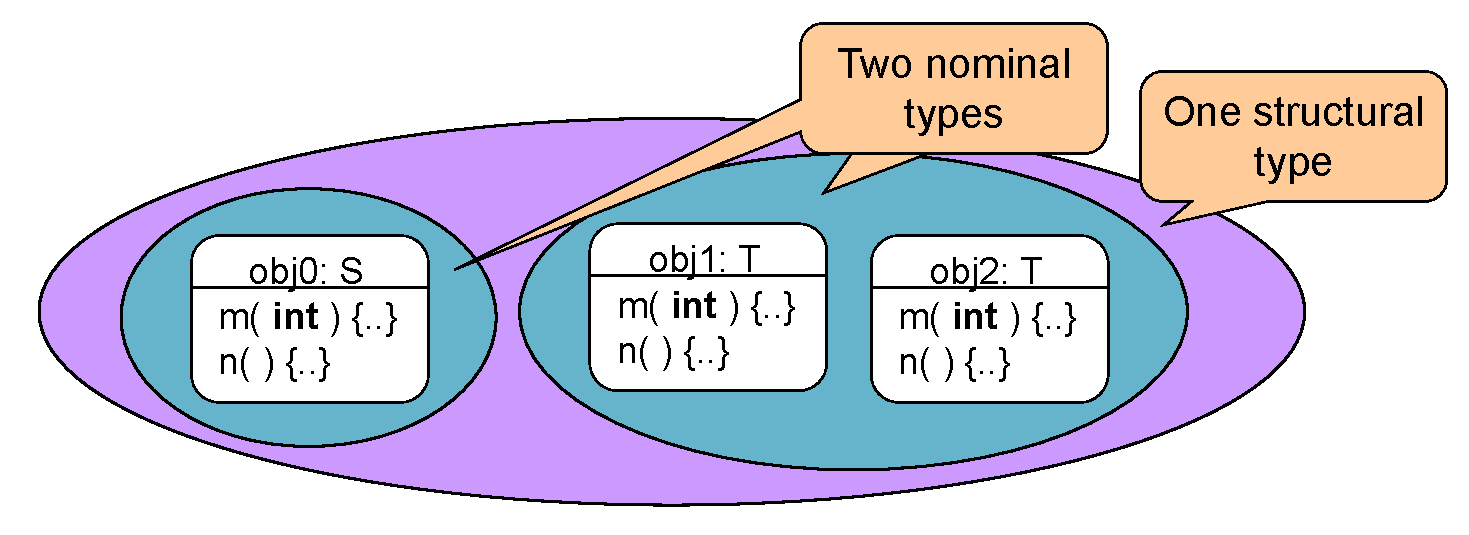
\includegraphics[width=0.7\textwidth]{img/02_nominal_types}
      \caption{Type Membership}
\end{figure}

\subsubsection{Example}

\lstset{language=C}
\begin{lstlisting}
class S {
  m( int ) { ... }
  n( )     { ... }
}

class T {
  m( int ) { ... }
  n( )     { ... }
}
\end{lstlisting}
\begin{itemize}
 \item \textbf S and \textbf T are \emph{\textbf{different} in nominal systems}
 \item \textbf S and \textbf T are \emph{\textbf{equivalent} in structural systems}
\end{itemize}

\subsection{Static Type Checking}
\emph{Each expression} of a program \emph{has a type}. \emph{Types} of variables and methods are \emph{declared explicitly} or \emph{inferred}. Types of expressions can be derived from the types of their constituents. \emph{Type rules} are used \emph{at compile time} to check whether a program is \emph{correctly typed}.
\paragraph{Examples: } $\text{}$
\begin{lstlisting}[caption=compiles]
int a;
boolean equals(Object o)
a + 7
"A number: " + 7
"A string".equals(null)
\end{lstlisting}
\begin{lstlisting}[caption=results in compile-time errors]
a = "A string";           // Assignment of a String to an integer
"A string".equals(1, 2);  // Too many arguments
\end{lstlisting}

\subsection{Dynamic Type Checking}
\emph{Variables}, \emph{methods}, and \emph{expressions} of a program \emph{are} typically \emph{not typed}. Every object and value has a type. A \emph{Run-time system} checks that operations are applied to \emph{expected arguments}.

\subsection{Static Type Safety}
\begin{definition}[Static Type Safety]
 A programming language is called type-safe if its design prevents type errors. 
\end{definition}
% Statically type-safe object-oriented languages
% \paragraph{Guarantees}: Statically type-safe object oriented languages guarantee the following invariant:
\begin{shadequote}
 In every execution state, the type of the value held by variable v is a subtype of the declared type of v.
\end{shadequote}
Most static type systems rely on dynamic checks for certain operations. Such as \emph{type conversion by casts}. \emph{Run-time checks} throw an exception in case of a type error.

\begin{lstlisting}[caption=Java example on a dynamic check]
Object[] oa = new Object[10];
String s    = "A String";
oa[0]       = s;
// ..
if (oa[0] instanceof String) {
  s = (String) oa[0];
}
s = s.concat("Another String");
\end{lstlisting}

Static checkers need to \emph{approximate run-time behavior} (conservative check). 
\lstset{language=Python}
\begin{lstlisting}[caption=Python example on dynamic type checking]
def divide(n,d):
  if d != 0:
    res = n/d
  else:
    res = "Division by zero"
  print res
\end{lstlisting}

Dynamic checkers support \emph{on-the-fly code generation} and dynamic class loading.
\lstset{language=Java}
\begin{lstlisting}[caption=JavaScript example on on-the-fly code generation]
eval (
  "x=10; y=20; document.write(x*y);"
);
\end{lstlisting}

\subsection{Comparison}

\subsection{Advantages of static checking}
\begin{description}
 \item[Static safety:] More errors are found at compile time.
 \item[Readability:] Types are excellent documentation.
 \item[Efficiency:] Type information allows optimizations.
\end{description}
\subsection{Advantages of dynamic checking}
\begin{description}
 \item[Expressiveness:] No correct program is reject by the type checker.
 \item[Low overhead:] No need to write type annotations.
 \item[Simplicity:] Static type systems are often complicated.
\end{description}

\begin{tabular}{r|p{5cm}p{5cm}}
& \textbf{Static} & \textbf{Dynamic}\\ \hline
\textbf{Nominal} & C++, C\#, Eiffel, Java, Scala & For certain features of statically-typed languages.\\
\textbf{Structural}& Research languages such as Moby, PolyToil, O'Caml. & JavaScript, Python, Ruby, Smalltalk.
\end{tabular}\\

Dynamically typed languages with a structural types are also called \emph{duck typed languages}.

\section{Subtyping}

\begin{shadequote}
  Objects of subtypes can be used wherever objects of supertypes are expected.\par\emph{Substitution principle}
\end{shadequote}

\begin{description}
 \item[Syntactic classification] Subtype objects can \emph{understand at least the messages} that supertype objects can understand.
 \item[Semantic classification] Subtype objects \emph{provide at least the behavior} of supertype objects.
\end{description}

The \emph{subtype relation} corresponds to the \emph{subset relation} on the values of a type.
\begin{figure}[h!]
  \centering
    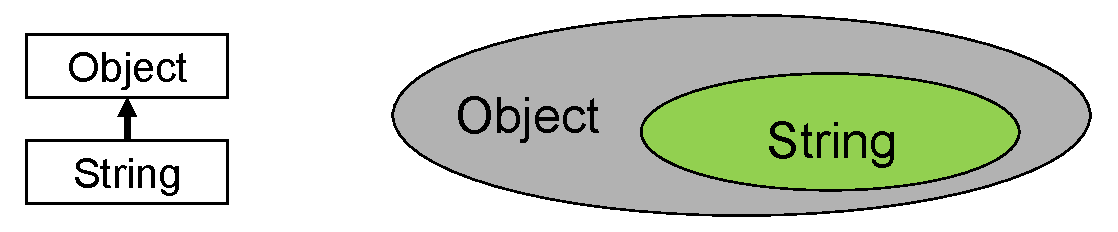
\includegraphics[width=0.5\textwidth]{img/02_subtype_relation}
%       \caption{Core Requirements in Software Technology}
\end{figure}

\begin{description}
 \item[Nominal type systems] Determine \emph{type membership} based on \emph{type names} and determine \emph{subtype relations} based on \emph{explicit declarations}:
 \lstset{language=Java}
 \begin{lstlisting}[caption=nominally typed language]
  class S { 
    m(int) {...} 
  }
  class T extends S { // nominal subtype because of extend declaration
    m(int) {...} 
  }
  class U {           // not a subtype of S
    m(int) {...}
    n()    {...}
  }
 \end{lstlisting}
  \item[Structural type systems] Determine \emph{type membership} and \emph{subtype relations} based on \emph{availability of methods and fields}:
  \begin{lstlisting}[caption=structurally typed language]
  class S {
    m(int) {...]
  }
  class T {         // Subtype of S
    m(int) {...}
  }
  class U {         // Subtype of U
    m(int) {...}
    n()    {...}
  }
  \end{lstlisting}

\end{description}

\subsection{Nominal Subtyping and Substitution}
Subtype objects can \emph{understand at least the messages} that supertype objects can understand:
\begin{itemize}
 \item Method calls
 \item Field accesses
\end{itemize}
Subtype objects have \emph{wider interfaces} than supertype objects:
\begin{itemize}
 \item Existence of methods and fields
 \item Accessibility of methods and fields
 \item Types of methods and fields
\end{itemize}

\subsubsection{Rules}
\begin{description}
 \item[Existence] \emph{Subtypes may add, but not remove methods and fields}
 \item[Accessibility] An \emph{overriding method must not be less accessible} than the methods it overrides:
 \begin{lstlisting}
  class Super {
    public void foo() {...}
    public void bar() {...}
  }
  
  class Sub <: Super {
    public void foo() {...}
    private void bar() {...} 
  }
  
  void m( Super s) { s.bar(); }
 \end{lstlisting}
 At run time, \lstinline{m} could access a private method of \lstinline{Sub}, thereby violating information hiding.
 \item[Contravariant parameters] An \emph{overriding method must not require \textbf{more specific} parameter types} than the method it overrides.
 \item[Covariant results] An \emph{overriding method must not have \textbf{more genera} result type} than then the ethod it overrides. 
 \item[Fields] \emph{Subtypes must not change the type of fields}
 	Regard field as pair of getter and setter methods:
 	\begin{itemize}
 		\item \emph{Specializing a field type} \lstinline{S<:T} corresponds to specializing the argument of the setter (\emph{violates the contravariant parameters})
 		\item \emph{Generalizing a field type} \lstinline{T<:S} corresponds to generalizing the result of the getter (\emph{violates covariant results}).
 		
 	\end{itemize}
 \item[Immutable Fields] Immutable fields do not have setters. \emph{Types of immutable fields can be specialized in subclasses} \lstinline{S<:T}. This only works in the absence of inheritance. 
 \item[Covariant Arrays] In Java and C\# \emph{arrays are covariant}. If \lstinline{S<:T} then \lstinline{S[] <: T[]}. Each \emph{array update requires} a \emph{run-time check}. Covariant arrays allow one to write methods that work for all arrays  such as:
 	\begin{lstlisting}
 	Class Arrays {
 		public static void fill(Object[] a, Object val) { ... }
 	}
 	\end{lstlisting}
	Generics allow a solution that is expressive and statically-safe. 
\end{description}

\subsection{Reuse: Adapter Pattern}
Nominal Subtyping can impede reuse.  Consider two library classes:
\begin{lstlisting}
class Resident {
	String 	getName( ) { ... } 
	Data 	dateOfBirth( ) { ... }
	Address	getAddress( ) { ... } 
}
class Employee {
	String 	getName( ) { ... } 
	Data 	dateOfBirth( ) { ... } 
	int		getSalary( ) { ... }
}
\end{lstlisting}
Now we would like to store Resident and Employee objects in a collection of type Person[]. Implement an Adapter:
\begin{itemize}
	\item Subtype of Person
	\item Delegate calls to adaptee
	\item Adapter requires boilerplate code
	\item Adapter causes memorz and run-time overhead
	\item Works also if Person is reused.
\end{itemize}

\begin{lstlisting}[caption=Adapter Pattern]
interface Person { 
	String 	getName(); 
	Data 	dateOfBirth();
}
class EmployeeAdapter implements Person { 
	private	Employee adaptee;
	String	getName() {
		return adaptee.getName(); 
	} 
	Data dateOfBirth() { 
		return adaptee.dateOfBirth(); 
	}
}
\end{lstlisting}

\subsection{Generalisation}
Most OO-languages support specialisation of superclasses (top-down development). Some research languages also support \emph{generalisation} (bottom-up development).
\begin{lstlisting}
	interface Person generalizes Resident, Employee {
		String	getName();
		Data	dateOfBirth();
	}
\end{lstlisting}
A supertype can be declared after a subtypes have been implemented. 
Generalisation does not match well with inheritance: A Subclass-to-be already has a superclass.

%\subsection{Structural Subtyping and Substitution}
%Subtype objects can \emph{understand at least the messages} that supertype objects can understand:
%\begin{itemize}
%	\item Method calls
%	\item Field accesses
%\end{itemize}
%Structural subtypes have \emph{by definition wider interfaces} then their supertypes.

\subsection{Reuse: Structural Subtyping}
Subtype objects can \emph{understand at least the messages} that supertype objects can understand:
\begin{itemize}
	\item Method calls
	\item Field accesses
\end{itemize}
Structural subtypes have \emph{by definition wider interfaces} then their supertypes.

All types are "automatically" subtypes of types with smaller interfaces. No support for inheritance (like generalization). 
\begin{lstlisting}[caption=Structural Subtyping Example]
interface Person {
	String 	getName();
	Data	dateOfBirth();
}

class Resident {
	String 	getName()		{...}
	Data	dateOfBirth()	{...}
	...
}	

class Employee {
	String 	getName()		{...}
	Data	dateOfBirth()	{...}
	...
}

\end{lstlisting}
Person is a supertype of Resident and Employee. We observe that generalisation doesn't match well with inheritance.



\subsection{Shortcomings}
Nominal subtyping can impede code reuse. Consider these two library classes:
\begin{lstlisting}
class Resident {
	String	getName()		{ ... }
	Date	dateOfBirth()	{ ... }
	Address	getAddress()	{ ... }
}

class Employee {
	String	getName()		{ ... }
	Date	dateOfBirth()	{ ... }
	int		getSalary()		{ ... }
}
\end{lstlisting}
Now we would like to store Resident and Employee-objects in a collection of type Person[]. Neither Resident nor Employee is a subtype of Person. So we implement and Adapter:
\begin{itemize}
	\item Subtype of Person
	\item Delegate calls to adaptee (Resident or Employee)
\end{itemize}
\begin{lstlisting}
interface Person {
	String	getName()		{ ... }
	Date	dateOfBirth()	{ ... }
}
class EmployeeAdapter implements Person {
	private	Employee	adaptee;
	String 	getName() {
		return adaptee.getName(); 
	} 
	Data 	dateOfBirth() { 
		return adaptee.dateOfBirth(); 
	}
}
\end{lstlisting}
The adapter requires boilerplate code and causes memory and run-time overhead. The adapter works also if Person is reused.



